%=========================================================================
% Start of 
%=========================================================================
\preClass{Inverse Functions}

\begin{problem}
\item The height, in meters, of a certain tree is given by the
  relationship
  \begin{eqnarray*}
    h(t) & = & \frac{50\cdot t}{25+t},
  \end{eqnarray*}
  where $t$ is the time in years from when the seed was germinated. 
  \begin{subproblem}
  \item Make a sketch of the height of a tree as a function of time.
    \vfill
  \item A tree is measured, and it is estimated that its height is 5
    meters. How long ago did its seed germinate?
    \vfill
  \item A tree is measured, and it is estimated that its height is 10
    meters. How long ago did its seed germinate?  
    \vfill
  \item Determine the function that takes the height of the tree and
    then determines its time since germination.
    \vfill
  \end{subproblem}

  \clearpage

\end{problem}


\actTitle{Inverse Functions}
\begin{problem}
\item Two functions are defined in the following tables. Determine the
  values of each expression below. If a value does not exist write
  ``NA.''

  \begin{tabular}[h]{l||l|l|l|l|l}
    $x$    & 0 & 1 & 2 & 3 & 4 \\ \hline
    $f(x)$ & 2 & 6 & 5 & 1 & 4 \\
  \end{tabular} ~~~
  \begin{tabular}[h]{l||l|l|l|l|l}
    $x$    & 1 & 2 & 4 & 5 & 6 \\ \hline
    $g(x)$ & 3 & 3 & 2 & 9 & 4 \\
  \end{tabular}

  \begin{subproblem}
  \item $f(g(4))$
    \vfill
  \item $g(f(4))$
    \vfill
  \item $f^{-1}(g(4))$
    \vfill
  \item $f(g^{-1}(4))$
    \vfill
  \item $f^{-1}(g^{-1}(3))$
    \vfill
  \end{subproblem}

  \clearpage

\item Given the graphs of the two functions below determine the values
  of the expressions below the graph.

  \hspace{-2em}
  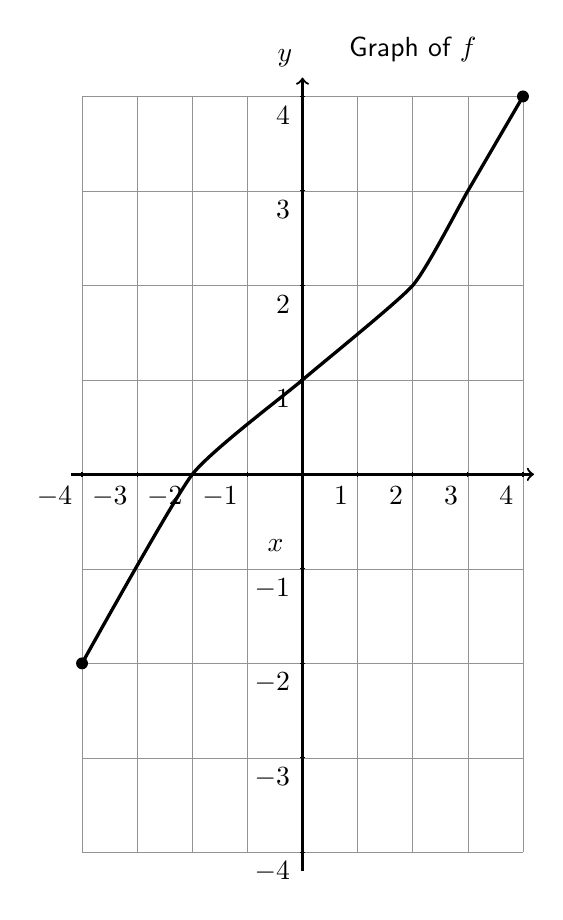
\begin{tikzpicture}[y=12mm, x=7mm,font=\sffamily]
    % ticks
    \draw[xstep = 1,ystep=1, gray, very thin,opacity=0.85] (-4, -4) grid (4, 4);
 	% axis
	\draw[thick,->] (-4.2,0) -- coordinate (x axis mid) (4.2,0) 
          node[yshift=-2em,xshift=-10em,anchor = north west] {$x$};
    \draw[thick,->] (0,-4.2) -- coordinate (y axis mid) (0,4.2) 
          node[anchor = south east] {$y$};
    \foreach \y in {-4,-3,-2,-1,1,2,3,4} {
      \draw (1pt, \y) -- (-1pt, \y) node[anchor = north east] {$\y$};
    }
    \foreach \x in {-4,-3,-2,-1,1,2,3,4} {
      \draw (\x,1pt) -- (\x,-1pt) node[anchor = north east] {$\x$};
    }
    % Draw the function
    \draw [black, very thick] plot [smooth, tension=0.3] coordinates {
      (-4,-2) (-2,0) (0,1) (2,2) (3,3) (4,4)};
    \fill[black] (-4,-2) circle [radius=0.5ex];
    \fill[black] ( 4, 4) circle [radius=0.5ex];
    \draw (2,4.5) node {Graph of $f$};
  \end{tikzpicture}
  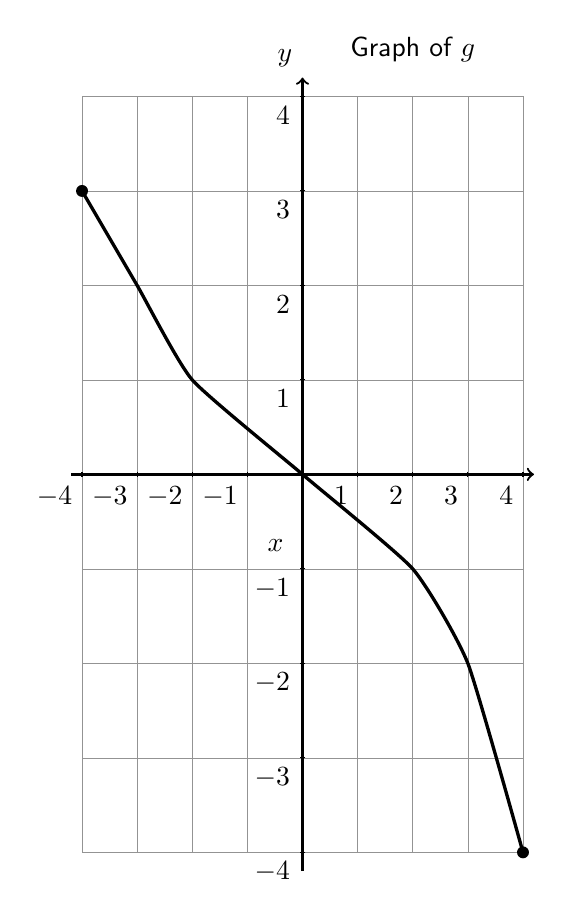
\begin{tikzpicture}[y=12mm, x=7mm,font=\sffamily]
    % ticks
    \draw[xstep = 1,ystep=1, gray, very thin,opacity=0.85] (-4, -4) grid (4, 4);
 	% axis
	\draw[thick,->] (-4.2,0) -- coordinate (x axis mid) (4.2,0) 
          node[yshift=-2em,xshift=-10em,anchor = north west] {$x$};
    \draw[thick,->] (0,-4.2) -- coordinate (y axis mid) (0,4.2) 
          node[anchor = south east] {$y$};
    \foreach \y in {-4,-3,-2,-1,1,2,3,4} {
      \draw (1pt, \y) -- (-1pt, \y) node[anchor = north east] {$\y$};
    }
    \foreach \x in {-4,-3,-2,-1,1,2,3,4} {
      \draw (\x,1pt) -- (\x,-1pt) node[anchor = north east] {$\x$};
    }
    % Draw the function
    \draw [black, very thick] plot [smooth, tension=0.3] coordinates {
      (-4,3) (-3,2) (-2,1) (0,0) (2,-1) (3,-2) (4,-4)};
    \fill[black] (-4, 3) circle [radius=0.5ex];
    \fill[black] ( 4,-4) circle [radius=0.5ex];
    \draw (2,4.5) node {Graph of $g$};
  \end{tikzpicture}


  \begin{subproblem}
    \item $f(g(3)) =$
      \vfill
    \item $f^{-1}(0) =$
      \vfill
    \item $f^{-1}(-2) = $
      \vfill
    \item $g^{-1}(f(0)) = $
      \vfill
  \end{subproblem}

\clearpage

\item The height, in meters, of a certain tree changes by the
  relationship
  \begin{eqnarray*}
    h(t) & = & \frac{50\cdot t}{25+t},
  \end{eqnarray*}
  where $t$ is the time in years from when the seed was germinated.
  \begin{subproblem}
    \item Determine the range and the domain of $h(t)$. (For the
      domain also consider the physical description as well as the
      definition of the function.)
      \vfill
    \item Determine the inverse of $h(t)$. How can it be interpreted?
      \vfill
    \item Determine the range and the domain of the inverse of $h(t)$.
      \vfill
  \end{subproblem}

  \clearpage

\item For each function below determine if it is one-to-one. For each
  function that is one-to-one determine the inverse of the
  function. For each function that is not one-to-one determine a
  subset of the domain for which the function is one-to-one on that
  subset. 
  \begin{subproblem}
    \item $f(x)=3x+1$
      \vfill
    \item $f(x)=\frac{1}{1+x}$
      \vfill
    \item $f(x)=x^2$
      \vfill
    \item $f(x)=\sqrt{3x+1}$
      \vfill
  \end{subproblem}

  \clearpage


\item \label{question:snakeTemps} The impact of sex determination in Pine Snakes was explored in a
  paper in \textbf{The American Naturalist}.\footnote{\textit{Effects
      of Incubation Temperature on Sex Ratios in Pine Snakes:
      Differential Vulnerability of Males and Females}, Joanna Burger
    and R. T. Zappalorti, \textbf{The American Naturalist} Vol. 132,
    No. 4 (Oct., 1988), pp. 492-505.} It was found that if the
  temperature of the Pine Snake's eggs was kept constant then the
  sex ratio in the brood can be approximated using a linear function
  of the temperature. The data suggests the following estimate:
  \begin{eqnarray*}
    \mathrm{Sex~Ratio(temp.)} & \approx & 0.68\cdot\mathrm{temp.}-0.95.
  \end{eqnarray*}
  (The sex ratio is calculated by taking the number of male snakes and
  dividing by the number of female snakes in the brood.)

  \begin{subproblem}
  \item What is the largest possible domain that can be used for this
    function? Does this result make physical sense?
    \vfill
  \item What is the meaning for the inverse function? What is the
    domain and range of the inverse?
    \vfill
  \item Determine the inverse function.
    \vfill
  \item Sketch a graph of the function and its inverse function on the
    following page. Label your axes and annotate your plots.  
  \end{subproblem}

\end{problem}

\postClass

\begin{problem}
\item Briefly state two ideas from today's class.
  \begin{itemize}
  \item 
  \item 
  \end{itemize}
\item  We examine the function
	\begin{eqnarray*}
		f(x) & = & x^2.
	\end{eqnarray*}
  \begin{subproblem}
    \item Determine if the function is 1-1.
    \item Determine a restriction on the domain of $f$ so that the function 
	    is 1-1 on the restricted domain.
    \item Determine the inverse on the restricted domain.
  \end{subproblem}
\item  We examine the function
	\begin{eqnarray*}
		f(x) & = & x^2-4x.
	\end{eqnarray*}
  \begin{subproblem}
    \item Determine if the function is 1-1.
    \item Determine a restriction on the domain of $f$ so that the function 
	    is 1-1 on the restricted domain.
    \item Determine the inverse on the restricted domain.
  \end{subproblem}
\end{problem}


%%% Local Variables:
%%% mode: latex
%%% TeX-master: "../labManual"
%%% End:

